\section{One-Factor Short-Rate Model}
As we have established, interest rate is crucial 
for pricing swaptions. Therefore, this chapter will 
begin by examining the general one-factor short rate 
model. It will then continue with a closer look at the 
Vasicek model, where we will determine its properties. 
To support and investigate these properties, a small 
simulation analysis of the Vasicek model will be 
performed.
\\\\
The risk-free short rate, r, is sometimes referred to as the instantaneous short rate. 
The concept is used in finance modeling to represent the continuously compounded interest rate for 
short time intervals. The short rate, r, is often modeled using stochastic deferential equations in 
mathematical finance. Some typically models for modeling the short rate is the Vacisek model and the Cox–Ingersoll–Ross model, 
later the Vacisek model will be covered. When pricing derivatives as bonds and options, the price depends on 
the process followed by r in the risk-neutral world \cite{Hull}.
\\\\
As discussed in the Section \ref{risk_neutral_section} - Risk Neutral Measure, $r_t$, can be looked at the locally risk-free 
rate from a continuously compounded bank account $B(t)= \exp \Big[\int_{0}^{t} r(s) ds \Big]$. 
Where the bank account has the dynamic listed in \autoref{bank1} and \autoref{bank2}.
Postulation the considered market is arbitrage-free, with due to the First Fundamental Theorem of Asset Pricing, 
if stating that there exist a probability measure $\QQ$, equivalent to $\PP$, all asset prices discounted by $B(t)$
are $\QQ$-martingales. In other words under the considered market for any T we have that 
\begin{align}
    \frac{P(0,T)}{B(0)} = P(0,T) = \EE^{\QQ} \Big( \frac{P(T,T)}{B(T)}\Big) = \EE^{\QQ} \Big( \frac{1}{B(T)}\Big) 
    = \EE^{\QQ} \Big( \exp \Big[ - \int_{0}^{t}r(s)ds \Big] \Big)
    \label{dist}
\end{align}
where $P(0,T)$ is the price at time zero of the asset and note that $P(T,T)=1$. So \autoref{dist} says that 
the time zero price of the asset are $\QQ$-expectations  of the payoff \cite{Bermudan}.
In other words in a market free of arbitrage, bond prices are determined by the risk-neutral expectations 
of how the short-term interest rate will behave. Because all types of interest rate instruments are based
on bond prices, the entire term structure or zero coupon curve can be described by the distributional properties
of just one state variable - the short rate \cite{Bermudan}.

\subsection{The Vasicek model}
So all interest rate instruments are fundamentally dependent on bond prices. Understanding the movements of 
these prices is essential for accurately describing the term structure or zero coupon curve. The behavior 
of the short rate, a key variable, underlies this understanding due to its distributional properties.
\\\\
The Vasicek model, introduced by Oldrich Vasicek in 1977, serves as a robust framework to analyze these dynamics.
The Vasicek model is renown for its simplicity and the ease with which it facilitates bond price calculations, 
the model assumes that the short-term interest rate adheres to a mean-reverting stochastic process. This process is characterized 
by parameters that dictate the rate's mean reversion speed, its long-term average level, and its volatility.
The model is used for forecasting how interest rates in the market will develop in the future. The model is a
mathematical result of interest rates and it is a one-factor short rate model and the model is constructed in the 
term of that the evolution of interest rates only depends on one stochastic variable.
\\\\
So now a short introducing to the Vasicek model has been covered and the next step is to look closer at the 
mathematical framework of the Vasicek model. The Vasicek model consists of the dynamic of the short rate under the $\PP$-measure
(the real world measure). Where the dynamic of the short rate is governed by a stochastic differential equation. 
The dynamic for the short rate in the Vasicek model is present below in \autoref{vas_dyn} and \autoref{vas_dyn_r0} \cite{Bjork}.
\begin{align}
    d r_t &= \kappa \Big[\theta -r(t)\Big] dt + \sigma d W(t) \label{vas_dyn}\\
    r(0) &= r_0 \label{vas_dyn_r0}
\end{align}
The dynamic for the short rate in \autoref{vas_dyn} is a Ornstein-Uhlenbeck process, which is a type of stochastic 
differential equation that describes the evolution of a mean-reverting behavior. So the process is consisting of a 
tendency to revert towards the mean of the process. This tendency is illustrated in \autoref{fig:vasicek} below, where 
 rates is simulated using the Vasicek model for some chosen parameters listed in \autoref{tab:parameters_short_rate} below. 
 Note in \autoref{fig:vasicek}
one simulated path of the short rate is illustrated. Where in \autoref{fig:vasicek-sim} ten simulated paths are illustrated,
but the same tendency appears. The parameters in the short rate dynamic
$\kappa$, $\theta$ and $\sigma$ are positive constants. Where $\kappa$ represent the mean reversion speed, $\theta$ 
is the long-term average rate, $\sigma$ is the volatility  and $W(t)$ is a Wiener process \cite{Bermudan}. 
\begin{table}[H]
    \centering
    \begin{tabular}{ccc}
      \toprule
      \textbf{Parameter} & \textbf{Parameter explanation} & \textbf{Value} \\
      \midrule
      $T$ & Time to maturity & 10 \\
      $r_0$ & Initial short rate & 0.05 \\
      $\kappa$ & Mean reversion speed & 0.2\\
      $\theta$ & Long-term average rate  & 0.03 \\
      $\sigma$ & Volatility& 0.02 \\
      \bottomrule
    \end{tabular}
    \caption{Summary of Parameters used for simulation short rate in the Vacisek model}
    \label{tab:parameters_short_rate}
\end{table}
\noindent
\begin{figure}[H]
    \centering
    \begin{minipage}{0.5\textwidth}
        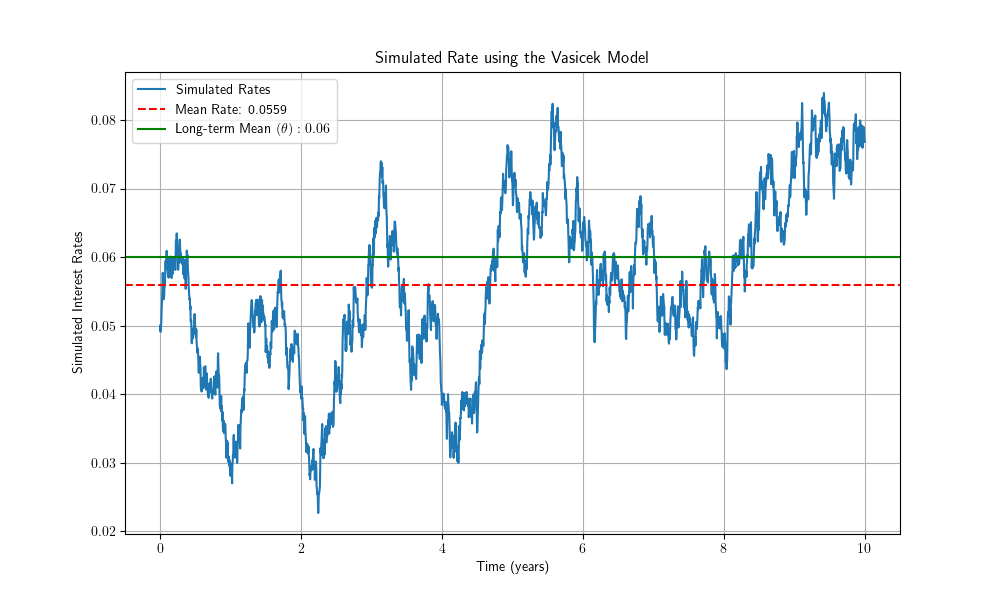
\includegraphics[width=\linewidth]{/Users/nannaingemannohrt/Desktop/master_thesis/main/plots/VasicekModelPlot.png}
        \caption{Plot of one simulated rate path \\ using the Vasicek model.}
        \label{fig:vasicek}
    \end{minipage}\hfill 
    \begin{minipage}{0.5\textwidth}
        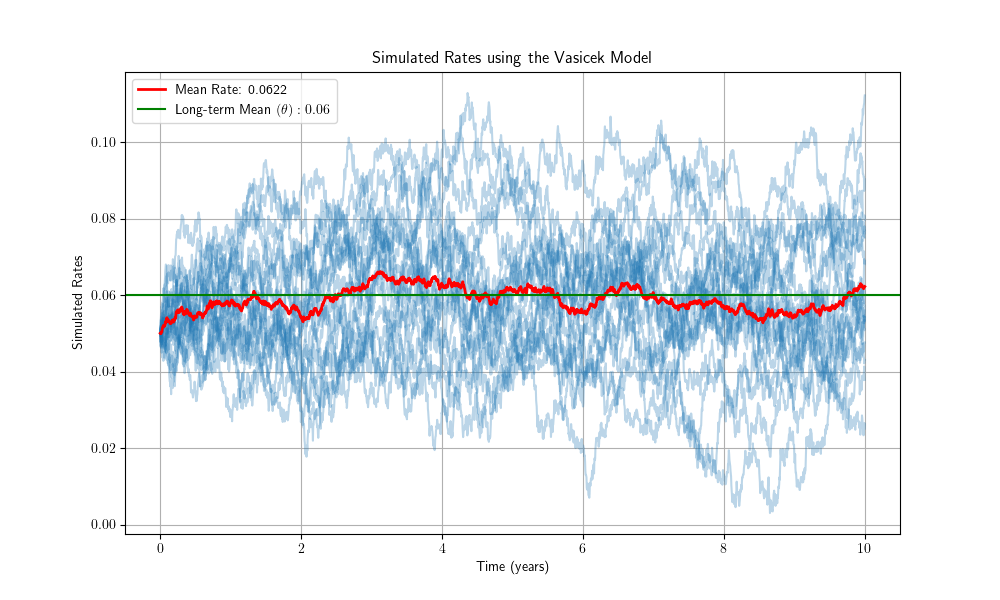
\includegraphics[width=\linewidth]{/Users/nannaingemannohrt/Desktop/master_thesis/main/plots/VasicekModelPlotSIM.png}
        \caption{Plot of 10 simulated  rates \\ paths using the Vasicek model.}
        \label{fig:vasicek-sim}
    \end{minipage}
\end{figure}
\noindent
Then we look closer at the dynamic of the short rate in \autoref{vas_dyn}. Which can be rearranged and integrated
to express the short rate, $r(t)$, as a function of its value at any prior time point s, 
so we have to have that for $s < t$ \cite{Bermudan}. 
\begin{align}
    d r_t &= \kappa \left[\theta - r(t)\right] dt + \sigma d W(t) \label{line_14} \\
    d r(t) &= k \theta dt - k r(t) dt + \sigma d W(t),  \\
    d r(t) + k r(t) dt &= k \theta dt + \sigma d W(t), \\
    e^{kt} d r(t) + k e^{kt} r(t) dt &= e^{kt} k \theta dt + e^{kt} \sigma d W(t), \\
    \frac{d}{dt} \left( e^{k t} r(t) \right) &= e^{k t} \frac{d}{dt} r(t) + k e^{k t} r_t dt, \\
    d\left( e^{k t} r(t) \right) &= e^{k t} dr(t) + k e^{k t} r_t dt, \\
    \int_s^t d \left( e^{ku} r(u) \right) &= k \theta \int_s^t e^{ku} du + \sigma \int_s^t e^{ku} d W(u), \\
    e^{kt} r(t) - e^{k s} r(s) &= \frac{k \theta}{k} \left( e^{kt} - e^{ks} \right) + \sigma \int_s^t e^{ku} d W(u), \\
    r(t) &= r(s) e^{-k(t-s)} + \theta \left( 1 - e^{-k(t-s)} \right) + \sigma \int_s^t e^{-k(t-u)} d W(u). \label{line_22}
\end{align}
From \autoref{line_14} to \autoref{line_22} the expression for the short rate in the Vasicek model is integrated, 
but first the terms in the stochastic differential equation is rearranged.
Then both sides of the equation are multiplied by the 
integrating factor $e^{\kappa t}$ to facilitate integration. Next both sides is integrated from s to t. The result of the
integration showing the change in the short  rate, r, over time, adjusted by the integrating factor. The final 
expression in \autoref{line_22} for the short rate, $r(t)$, at time t, showing how it depends on the initial rate, $r(s)$,
the mean-reverting term and the stochastic term \cite{Bermudan}. We note that  final expression in \autoref{line_22} for the short rate
is Gaussian.
\\\\
Further we find that $r(t)$ is normally distributed with mean and variance determined as follows \cite{Bjork}. 
\begin{align*}
    \EE \Big[r(t)\Big] & = \EE \Big[ r(s) e^{-k(t-s)} \Big] + \EE \Big[\theta \left( 1 - e^{-k(t-s)} \right)\Big]
    + \underset{:=0}{\underbrace{\EE \Big[\sigma \int_s^t e^{-k(t-u)} d W(u)\Big] }}\\
    & = \EE \Big[ r(s) e^{-k(t-s)} \Big] + \EE \Big[\theta \left( 1 - e^{-k(t-s)} \right)\Big] \\
    & = r(s) e^{-k(t-s)} + \theta \left( 1 - e^{-k(t-s)} \right) 
\end{align*}    
Using stochastic calculus, it can be demonstrated that the stochastic integral of a deterministic function 
$f(s)$ with respect to a Wiener process is distributed according to a Gaussian distribution,
having a mean of zero and a variance given by $\int_0^t f(s) ds$. We use this to find the variance of the short rate,
$r(t)$ \cite{Bjork}.
\begin{align*}
    Var\Big[r(t)\Big] &= Var\Big[\sigma \int_{s}^{t}e^{-k(t-u)} d W(u) \Big] \\
    &= \sigma^2 \int_{s}^{t}e^{-2k(t-u)} d W(u) \\
    &= \frac{\sigma^2}{2\kappa} \Big(e^{-2k(t-s)}\Big)
    \end{align*}
This lead to the theoretical distributed of the the short rate in the Vasicek model, which is represent below
\begin{align}
    R(t) \sim \mathcal{N} \Big[ r(s) e^{-k(t-s)} + \theta \left( 1 - e^{-k(t-s)} \right) ,
    \frac{\sigma^2}{2\kappa} \Big(e^{-2k(t-s)}\Big) \Big]
\end{align}
Mowing toward simulating the distribution, we can use the above attributes of the short rate being Gaussian.
Given that the stochastic integral of a deterministic function with respect to a Wiener process is Gaussian distributed
with a mean of zero, we can simulate the short rate distribution by generating a large number of possible paths
for the Wiener process. Each path would then correspond to a realization of the short rate over time. In \autoref{fig:rates:hist}
below the described method is used and the simulated path for the short rate in the Vasicek model and the distributed of one  the
simulated paths is plotted in a histogram. In \autoref{fig:rates:hist} the probability density function (PDF) of the 
fitted normal distribution is also plotted. This verify that the short rate process in the Vasicek model is Gaussian distributed.
\begin{figure}[H]
    \centering
    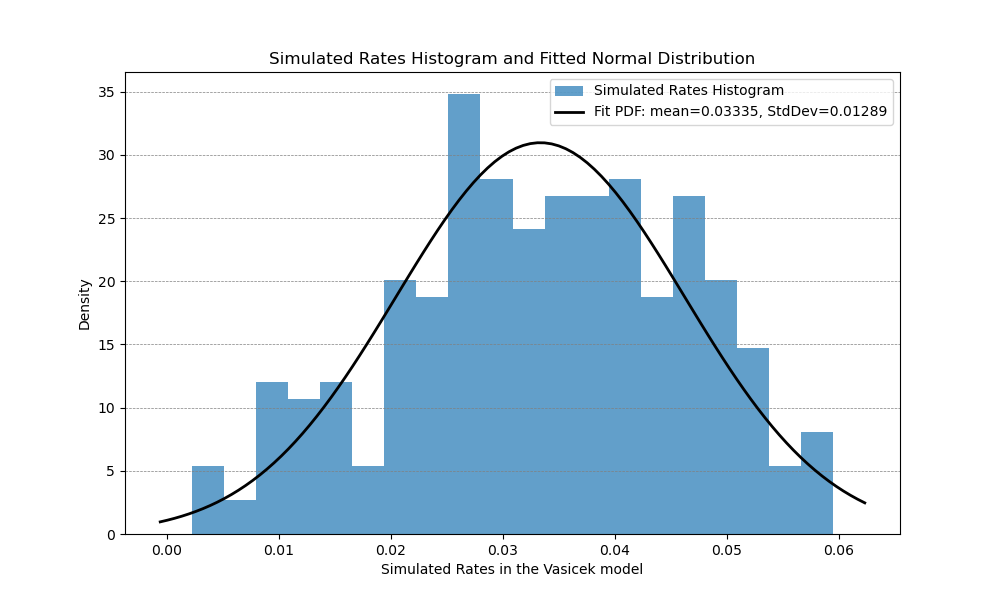
\includegraphics[width=0.7\textwidth]{/Users/nannaingemannohrt/Desktop/master_thesis/main/plots/NormalDistributionPlot.png}
    \caption{Histogram of one simulated rates path using the Vasicek model.}
    \label{fig:rates:hist}
\end{figure}
\noindent
Now some common properties of the Vasicek model has been reviewed and supported by simulations. Mowing forward we will 
focus on bond prices using the Vasicek model. Earlier when we discussed bond prices, the Black Scholes model was introduced. 
\\\\
Now we will examine another aspect of the Vasicek model, namely the ability to derive explicit formulas
for bons pricing based on model expectations.
But first some words on how these bond prices is determine in the Vasicek model. 
When using the Vasicek model, it is possible to derive closed-form solutions for zero coupon bond prices. 
These prices are determined by an equation that factors in the current short rate, the speed of mean reversion,
the long-term mean rate, the volatility of the short rate, and the bond’s time to maturity.
The bond prices formula from the Vasicek model considers the expected path of future short 
rates under the risk neutral measure, discounted back to the present value. 
\\\\
As mentioned we will now look a the formula for pricing bond using the Vasicek model. We consider a zero coupon bond
with maturity T and at time t the price is given as in \autoref{price_zcb_vas} below \cite{Bjork}.
\begin{align}
    P(t,T) &= A(t,T) e^{-rB(t,T)} 
    \label{price_zcb_vas} 
\end{align}
Then we find the partial derivatives with respect to $r$ and $t$ of the zero coupon bond listed in \autoref{price_zcb_vas}.
\begin{align*}
    \frac{\partial P}{\partial t} &= \frac{\partial}{\partial t} (Ae^{-rB}) 
    = e^{-rB} \frac{\partial A}{\partial t} + Ae^{-rB} \frac{\partial}{\partial t} (-rB) \\
    &= e^{-rB} \frac{\partial A}{\partial t} - rAe^{-rB} \frac{\partial B}{\partial t} = 
    - \frac{P}{A} \frac{\partial A}{\partial t} - rP \frac{\partial B}{\partial t}
    \\\\
    \frac{\partial P}{\partial r} &= \frac{\partial}{\partial r} (Ae^{-rB}) 
    = Ae^{-rB} \frac{\partial}{\partial r} (-rB) = -PB 
    \\\\
    \frac{\partial^2 P}{\partial r^2} &= \frac{\partial}{\partial r} (-PB) = -B \frac{\partial}{\partial r} (P) = PB^2
\end{align*}
Then by applying Ito's lemma \cite{Bjork} and insetting the derivatives with respect to $r$ and $t$ we found above and
insetting the formula for the short rate in the Vasicek model present in \autoref{vas_dyn} we obtain the following
\begin{align*}
    dP(t,T) &= \frac{\partial P}{\partial t} dt + \frac{\partial P}{\partial r} dr 
    + \frac{1}{2} \frac{\partial^2 P}{\partial r^2} dr^2 \\
    dP(t,T) &= \left( \frac{P}{A} \frac{\partial A}{\partial t} - rP \frac{\partial B}{\partial t} \right) dt 
    + (-PB) dr + \frac{1}{2} (PB^2) dr^2 \\
    \frac{dP}{P} &= \left( \frac{1}{A} \frac{\partial A}{\partial t} - r \frac{\partial B}{\partial t} \right) dt 
    - B dr + \frac{1}{2} B^2 dr^2 \\
    \frac{dP}{P} &= \left( \frac{1}{A} \frac{\partial A}{\partial t} - r \frac{\partial B}{\partial t} \right) dt
     - B(\kappa \theta dt - \kappa r dt + \sigma dW_t) + \frac{1}{2} B^2 \sigma^2 dt\\
    \frac{dP}{P} &= \left( \frac{1}{A} \frac{\partial A}{\partial t} - r \frac{\partial B}{\partial t} 
    - \kappa \theta B + \kappa r B + \frac{1}{2} B^2 \sigma^2 \right) dt - \sigma B dW_t \\
\end{align*}
Under the risk neutral measure, the expected return of the bond must be equal to the risk free rate. Thus we have that
\begin{align*}
    r  &= \frac{1}{A} \frac{\partial A}{\partial t} - r \frac{\partial B}{\partial t} - \kappa \theta B 
    + \kappa r B + \frac{1}{2} B^2 \sigma^2  \\
    r \left( 1 + \frac{\partial B}{\partial t} - \kappa B \right) & =\frac{1}{A} \frac{\partial A}{\partial t} 
    - \kappa \theta B + \frac{1}{2} B^2 \sigma^2 
\end{align*}
Since this holds for all values of $r$, which does not feature in the left hand side, we deduce that
\begin{align}
    0 &= \frac{1}{A} \frac{\partial A}{\partial t} - \kappa \theta B + \frac{1}{2} B^2 \sigma^2 \label{equal_zero2}\\
    0 &=1 + \frac{\partial B}{\partial t} - \kappa B \label{equal_zero}
\end{align}
Considering that the price of zero coupon bond at maturity $P(T,T)=1$, the function $P=A e^{-rB}$ suggests $B(T,T)=0$
and $A(T,T)=0$. By then applying the integrating factor to the \autoref{equal_zero}, reorganizing and integrating
form t to T, we obtain
\begin{align}
   0 &= 1 + \frac{\partial B}{\partial t} - \kappa B \nonumber  \\
   0 &= e^{-\kappa t} + e^{-\kappa t} \frac{\partial B}{\partial t} - e^{-\kappa t} \kappa B \nonumber \\
   -e^{-\kappa t} &= e^{-\kappa t} \frac{\partial B}{\partial t} - e^{-\kappa t} \kappa B  \nonumber \\
   -e^{-\kappa t} dt &= d \left( e^{-\kappa t} B(t, T) \right) \nonumber \\
   - \int_{t}^{T} e^{-\kappa u} du &= \int_{t}^{T} d \left( e^{-\kappa t} B(t, T) \right) \nonumber  \\
   \frac{1}{\kappa} \left( e^{-\kappa T} - e^{-\kappa t} \right) &= e^{-\kappa T} B(T, T) - e^{-\kappa t} B(t, T)\nonumber  \\
   B(t,T) & =\frac{1}{\kappa} \left( 1 - e^{-\kappa (T-t)} \right)  
\end{align}
Finally  by substituting into \autoref{equal_zero2} and integrating we get that
\begin{align}
    0 &=\frac{1}{A} \frac{\partial A}{\partial t} - \kappa \theta B + \frac{1}{2} B^2 \sigma^2 \nonumber \\
    0 &= \frac{1}{A} \frac{\partial A}{\partial t} - \kappa \theta \left( \frac{1 - e^{-\kappa(T-t)}}{\kappa}
    \right) + \frac{\sigma^2}{2\kappa^2} \left( 1 - e^{-\kappa(T-t)} \right)^2 \nonumber \\
    0 &=  \frac{1}{A} \frac{\partial A}{\partial t} - \theta \left( 1 - e^{-\kappa(T-t)} \right) 
    + \frac{\sigma^2}{2\kappa^2} \left( 1 + e^{-2\kappa(T-t)} - 2e^{-\kappa(T-t)} \right)\nonumber \\
    \frac{1}{A} \frac{\partial A}{\partial t} &€= \theta \left( 1 - e^{-\kappa(T-t)} \right) 
    - \frac{\sigma^2}{2\kappa^2} \left( 1 + e^{-2\kappa(T-t)} - 2e^{-\kappa(T-t)} \right) \nonumber\\
    \int_{t}^{T} \frac{dA(u, T)}{A(u, T)} &= \theta \int_{t}^{T} \left(1 - e^{-\kappa(T-u)}\right) du 
    - \frac{\sigma^2}{2\kappa^2} \int_{t}^{T} \left(1 + e^{-2\kappa(T-u)} - 2e^{-\kappa(T-u)}\right) du \nonumber\\
    \ln A(T, T) - \ln A(t, T) &= \theta (T - t) - \theta \left(\frac{1 - e^{-\kappa(T-t)}}{\kappa} \right)
    - \frac{\sigma^2}{2\kappa^2} \left( (T - t) + \left(\frac{1 - e^{-2\kappa(T-t)}}{2\kappa}\right) 
    - 2\frac{1 - e^{-\kappa(T-t)}}{\kappa}\right) \nonumber\\
    -\ln A(t, T) &= \theta (T - t) - \theta \left(\frac{1 - e^{-\kappa(T-u)}}{\kappa} \right)
    - \frac{\sigma^2}{4\kappa^3} \left(2\kappa (T - t) + 1 - e^{-2\kappa(T-t)} - 4 + 4e^{-\kappa(T-t)}\right) \nonumber\\
    -\ln A(t, T) &= \theta (T - t) - \theta \left(\frac{1 - e^{-\kappa(T-u)}}{\kappa} \right)
    - \frac{\sigma^2}{4\kappa^3} \left(2\kappa (T - t) - \left(1 + e^{-2\kappa(T-t)} 
    - 2e^{-\kappa(T-t)}\right) - 2 + 2e^{-\kappa(T-t)}\right) \nonumber\\
    -\ln A(t, T) &= \theta (T - t) - \theta \left(\frac{1 - e^{-\kappa(T-u)}}{\kappa}\right) - \frac{\sigma^2}{2 \kappa^2}
    \left((T-t)- \frac{1-e^{-\kappa(T-t)}}{\kappa}\right) + \frac{\sigma^2}{4 {\kappa}^3}\left(1-e^{-\kappa(T-t)}\right)^2 \nonumber\\
    \ln A(t, T) &= \left(\theta -\frac{\sigma^2}{2\kappa^2}\right) \left(\frac{1-e^{-\kappa(T-u)}}{\kappa}-(T-t)\right)
    -\frac{\sigma^2}{4 \kappa}\left(\frac{1-e^{-\kappa(T-t)}}{\kappa}\right)^2 \nonumber\\
    A(t,T)&= \exp \Biggl\{\left(\theta-\frac{\sigma^2}{2 \kappa^2}\right)\left(\frac{1-e^{-\kappa(T-u)}}{\kappa}-(T-t)\right)
    -\frac{\sigma^2}{4 \kappa}\left(\frac{1-e^{-\kappa(T-t)}}{\kappa}\right)^2 \Biggr\} 
\end{align}
 Combining this we get the formula for pricing bonds using the Vasicek model, which present 
 in Proposition \autoref{prop 5} below. 
\begin{proposition}
    \label{prop 5}
    \textbf{(The Vasicek term structure)} In the Vasicek model, bond prices are given by
 \begin{align}
    P(t,T) &= A(t,T) e^{-rB(t,T)} 
\end{align}
where
\begin{align*}
    A(t,T)&= \exp \Biggl\{\left(\theta-\frac{\sigma^2}{2 \kappa^2}\right)\left(\frac{1-e^{-\kappa(T-u)}}{\kappa}-(T-t)\right)
    -\frac{\sigma^2}{4 \kappa}\left(\frac{1-e^{-\kappa(T-t)}}{\kappa}\right)^2 \Biggr\} \\
    B(t,T) & =\frac{1}{\kappa} \left( 1 - e^{-\kappa (T-t)} \right)  
\end{align*}
\cite{Bjork}

\end{proposition}
\noindent
To illustrate the behavior of bond price in the Vacisek model, a small simulation study is perform. For the study 
some parameters are chosen, these are listed in \autoref{tab:parameters_zcb}
\begin{table}[H]
    \centering
    \begin{tabular}{ccc}
      \toprule
      \textbf{Parameter} & \textbf{Parameter explanation} & \textbf{Value} \\
      \midrule
      $T$ & Time to maturity & 10 \\
      $r_0$ & Initial short rate & Simulated \\
      $\kappa$ & Mean reversion speed & 0.2\\
      $\theta$ & Long-term average rate  & 0.03 \\
      $\sigma$ & Volatility& 0.02 \\
      \bottomrule
    \end{tabular}
    \caption{Summary of Parameters used simulation ZCB prices in the Vacisek model}
    \label{tab:parameters_zcb}
\end{table}
\noindent
\begin{figure}[H]
    \centering
    \begin{minipage}{0.5\textwidth}
        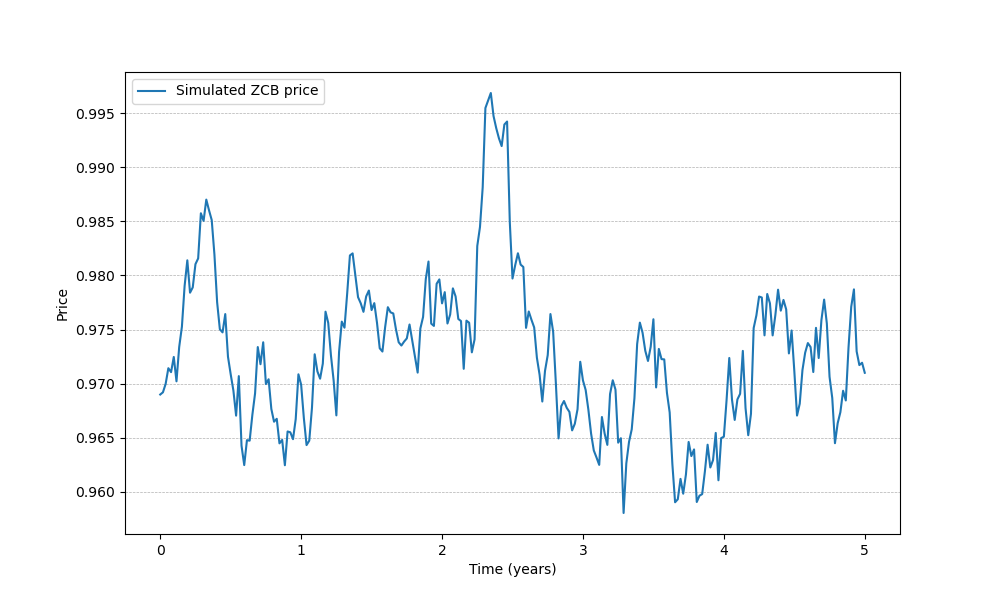
\includegraphics[width=\linewidth]{/Users/nannaingemannohrt/Desktop/master_thesis/main/plots/zcb_1_sim.png}
        \caption{Plot of one simulated ZCB price path \\ using the Vasicek model.}
        \label{fig:zcb_sim_1_plot}
    \end{minipage}\hfill 
    \begin{minipage}{0.5\textwidth}
        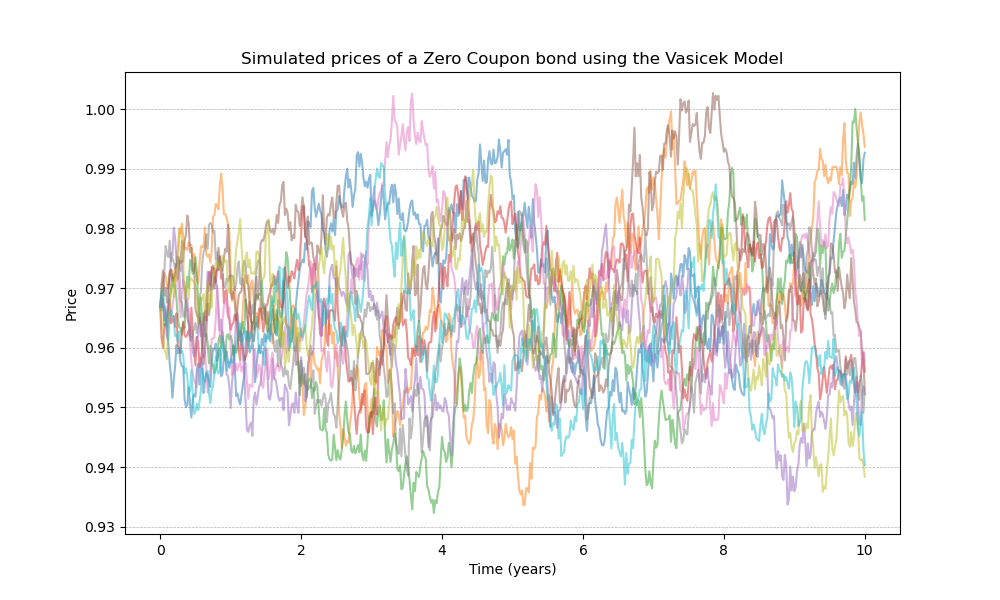
\includegraphics[width=\linewidth]{/Users/nannaingemannohrt/Desktop/master_thesis/main/plots/zcb_10_sim.png}
        \caption{Plot of 10 simulated  ZCB prices \\ paths using the Vasicek model.}
        \label{fig:zcb_sim_10_plot}
    \end{minipage}
\end{figure}
\noindent
\noindent
The Vasicek model has now been introduced and we have taken a closer look at the distribution in the short rate model. 
This examination leads us to the Vasicek term structure model, which outlines the method for pricing bonds using the 
Vasicek framework. Similarly, in Section 3, specific decisions are made regarding the calculation of bond prices with 
the Vasicek model. A critical decision is the assumption that the volatility, 
$\sigma$, is a positive constant. However, we should consider whether volatility remains constant over a given period.
\\\\
Subsequently, we will introduce another model, the SABR (Stochastic Alpha, Beta, Rho) model. The SABR model is a stochastic volatility model 
utilized to estimate the implied volatility curve. Although it does not provide a direct formula for option pricing, 
the estimated implied volatility curve can be employed in the Black Scholes model, discussed earlier, to price swaptions. 
Before we delve into the SABR model, we will examine the assumption of constant volatility inherent in the Black Scholes model.
The purpose of this small analysis, it to make a attachment to the
market and see some examples of not constant volatility. This can 
be seen as a motivation for looking into two-factor models, 
instead of a one-factor model, like the Vasicek model. 
